\section{ActiveClean: Machine Learning on Dirty Data}
Analytics is moving beyond SQL, and the growing popularity of predictive models \cite{bdas, alexandrov2014stratosphere, crotty2014tupleware, hellerstein2012madlib} leads to additional challenges in managing dirty data.
Predictive models rely on learning relationships between features and labels, and systematic corruption \cite{taylor1982introduction} (i.e., corruption that disproportionately affects certain data) can mask or even introduce spurious new relationships.
Furthermore, the high dimensionality of these models can amplify small problems \cite{xiaofeature} resulting in error-prone predictions even when trained on mostly clean data.
Our key insight is that predictive models are essentially high dimensional aggregate queries but that dimensionality leads to new challenges.

\subsection{Motivation}
Consider a music recommender system in which due to a software bug, all users from Europe have an incorrect age attribute defaulted to ``18-24".
A recommendation model trained on this data may spuriously learn a correlation relationship between age ``18-24" and music liked by European users.
A bug, which ostensibly affected only the European users' rows, can affect predictions to all users aged ``18-24".
Systematic corruption prior to featurization is not addressed in the robust Machine Learning literature which focuses on the resilience to outliers (e.g., age ``150").

Unfortunately, a straight-forward application of the techniques proposed in the previous sections have problems.
Consider the direct estimation technique for aggregate queries.
Accurate model training may require a large amount of training data and $k$ examples may not be enough for a viable model.
High-dimensional predictive models may actually be more sensitive to lack of training data than data error.
On the other hand, the correction technique and the bounds were derived for a small class of aggregates.
This does not generalize to an arbitrary statistical model. 
The goal of this work is to derive a scheme analogous to the correction technique but theoretically justified for predictive analytics.

\subsection{Simpson's Paradox}
The challenge is that the high-dimensional models are very sentitive to systematic biases, and many of the techniques applied in practice suffer methodological problems.
One technique to avoid dependence on sample size is ``write back" approach, where $k$ rows are cleaned and written back to the database.
Let $k$ rows be cleaned, but all of the remaining dirty rows are retained in the dataset.
Figure \ref{update-arch1} highlights the dangers of this approach on a very simple dirty dataset and a linear regression model i.e., the best fit line for two variables. 
One of the variables is systematically corrupted with a translation in the x-axis (Figure \ref{update-arch1}a).
The dirty data is marked in brown and the clean data in green, and their respective best fit lines are in blue.
After cleaning only two of the data points (Figure \ref{update-arch1}b), the resulting best fit line is in the opposite direction of the true model.
This is a well-known phenomenon called Simpsons paradox, where mixtures of different populations of data can result in spurious relationships \cite{simpson1951interpretation}.
Training models on a mixture of dirty and clean data can lead to unreliable results, where artificial trends introduced by the mixture can be confused for the effects of data cleaning.
Figure \ref{update-arch1}c also illustrates that, even in two dimensions, models trained from small samples can be as incorrect as the mixing solution described before.

\begin{figure}[ht!]
\centering
 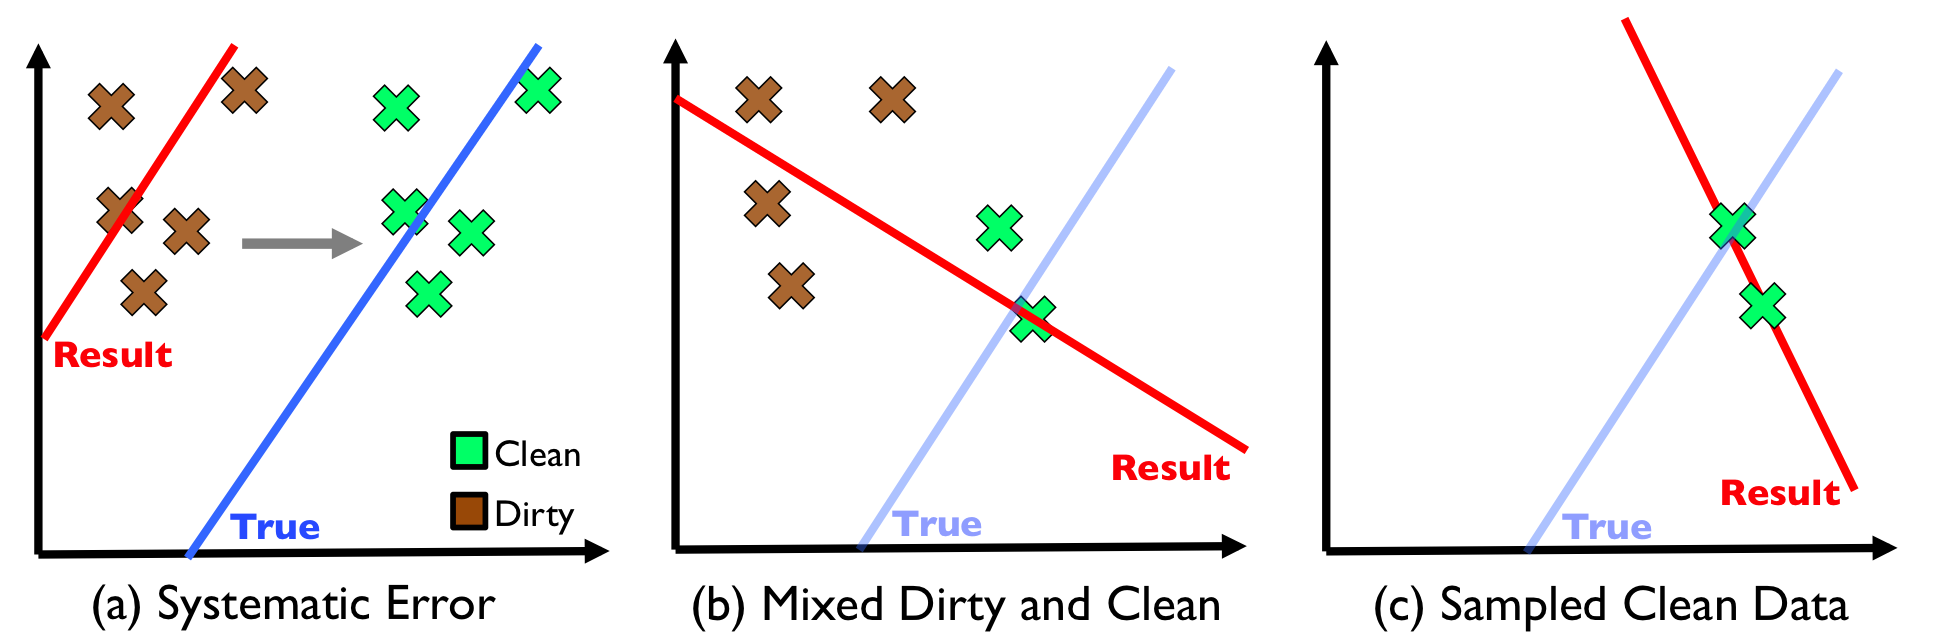
\includegraphics[width=0.6\columnwidth]{figs/update-arch.png}
 \caption{(a) Systematic corruption in one variable can lead to a shifted model. 
 (b) Mixed dirty and clean data results in a less accurate model than no cleaning.
(c) Small samples of only clean data can result in similarly inaccurate models. \label{update-arch1}}
\end{figure}

\subsection{Problem Setup}
This work focuses on a class of well analyzed predictive analytics problems; ones that can be expressed as the minimization of convex loss functions.
Examples includes all generalized linear models (including linear and logistic regression), all variants of support vector machines, and in fact, \avgfunc and \medfunc are also special cases. 

Formally, for labeled training examples $\{(x_{i},y_{i})\}_{i=1}^{N}$, the problem is to find a vector of \emph{model parameters} $\theta$ by minimizing a loss function $\phi$ over all training examples:
\[
 \theta^{*}=\arg\min_{\theta}\sum_{i=1}^{N}\phi(x_{i},y_{i},\theta)
\]
Where $\phi$ is a convex function in $\theta$.
Typically, a \emph{regularization} term $r(\theta)$ is added to this problem.
$r(\theta)$ penalizes high or low values of feature weights in $\theta$ to avoid overfitting to noise in the training examples.
\[
 \theta^{*}=\arg\min_{\theta}\sum_{i=1}^{N}\phi(x_{i},y_{i},\theta) + r(\theta)
\]
Without loss of generality, we will include the regularization as part of the loss function i.e., $\phi(x_{i},y_{i},\theta)$ includes $r(\theta)$.

\begin{definition}[Convex Data Analytics]
A convex data analytics problem is specified by a set of features $X$, corresponding set of labels $Y$, and a parametrized loss function $\phi$ that is convex in its parameter $\theta$.
The result is a \textbf{model} $\theta$ that minimizes the sum of losses over all features and labels.
\end{definition}

\vspace{0.5em}
\noindent\textbf{ActiveClean Problem: }\label{activeclean}\sloppy
Let $R$ be a dirty relation, $F(r) \mapsto (x,y)$ be a featurization that maps
a record $r \in R$ to a feature vector $x$ and label $y$, $\phi$ be a convex regularized loss,
and $C(r) \mapsto r_{clean}$ be a cleaning technique that maps a record to its cleaned value. 
Given these inputs, the ActiveClean problem is to return a \textbf{reliable} estimate $\hat{\theta}$ of the clean model for any limit $k$ on the number of times the data cleaning $C(\cdot)$ can be applied.

\vspace{0.25em}

\emph{Reliable} precisely means that the expected error in this estimate (i.e., L2 difference w.r.t a model trained on a fully cleaned dataset) is bounded above by a monotonically decreasing function in $k$ and a monotonically decreasing function of the error of the dirty model. In other words, more cleaning implies more accuracy, and less initial error implies faster convergence.

\subsection{Model Updates}
The main insight of this work is that, in Convex Data Analytics, sampling is natually part of the query processing.
Mini-batch stochastic gradient descent (SGD) is an algorithm for finding the optimal value
given the convex loss and data.
In mini-batch SGD, random subsets of data are selected at each iteration and the average gradient is computed for every batch.
Instead of calculating the average gradient for the batch w.r.t to the dirty data, we apply data cleaning at that point--inheriting the convergence bounds from batch SGD.
It is well known that even for an arbitrary initialization SGD makes significant progress in less than one epoch (a pass through the entire dataset) \cite{bottou2012stochastic}.
Furthermore in this setting, the dirty model can be much more accurate than an arbitrary initialization; leading to highly accurate models without processing the entire data.

ActiveClean is initialized with $\theta^{(1)} = \theta^{(d)}$ which is the dirty model.
At each iteration $t=\{1,...,T\}$, the cleaning is applied to a batch of data $b$ selected from the set of candidate dirty rows $R$.
Then, an average gradient is estimated from the cleaned batch and the model is updated.
Iterations continue until $k = T \cdot b$ rows are cleaned.

\begin{enumerate}[noitemsep]
	\item Calculate the gradient over the sample of clean data and call the result $g_S(\theta^{(t)})$
	\item Apply the following update rule:
	\[
	\theta^{(t+1)} \leftarrow \theta^{(t)} - \lambda \cdot g_S(\theta^{(t)}) 
	\]
\end{enumerate} 

\subsection{Optimizations}
ActiveClean has a number of additional optimizations exploiting the structure of Convex Data Analytics problems.

\noindent\textbf{Detector: } In this step, the detector select a candidate set of dirty rows $R_{dirty} \subseteq R$. There are two techniques to do this: (1) an \emph{a priori} case, and (2) and an adaptive case. In the \emph{a priori} case, the detector knows which data is dirty in advance. In the adaptive case, the detector learns classifier based on previously cleaned data to detect corruption in uncleaned data. This allows ActiveClean to prioritize cleaning data expected to be dirty. 

\vspace{0.5em}

\noindent\textbf{Non-uniform Sampler: } The sampler draws a sample of rows $S_{dirty} \subseteq R_{dirty}$. This is a non-uniform sample where each record $r$ has a sampling probability $p(r)$.
We derive the theoretical minimum variance sampling distribution, which is impossible to realize as it requires knowing the clean data in advance. Therefore, we use a first order first-order approximation of this distribution based on estimates of the clean data. 

\vspace{0.5em}

\noindent\textbf{Estimator: } The estimator approximates the optimal distribution derived in the Sample step. Based on the change in the featurized data $F(S_{clean})$ and $F(S_{dirty})$, it directs the next iteration of sampling to select points that will have changes most valuable to the next model update.



